\documentclass[11pt]{beamer}
\usetheme{Warsaw}
\usepackage[utf8]{inputenc}
\usepackage[spanish]{babel}
\usepackage{amsmath}
\usepackage{amsfonts}
\usepackage{amssymb}
\usepackage{graphicx}
\author{N.Pérez-Medina}
\title{Capítulo 5 - Inestabilidad: Exponentes de Lyapunov.}
\setbeamercovered{transparent} 
\setbeamertemplate{navigation symbols}{} 
\logo{
\includegraphics[scale=0.04]{logo_fing_uach_bn.png} } 
\institute{\textbf{FING - UACH}
	\\
	\begin{small}
	\textit{Resumen del libro 'Análisis de series de tiempo no lineales' de Kantz y Schreiber}\\
	\end{small}
	
	\bigskip
	
	\begin{small}
	\textbf{Catedrático:} Dr. José Luis Herrera Aguilar
	\end{small}		
	} 
\date{\today} 
\subject{Series de tiempo} 


% Para tener un morado coqueto
\definecolor{lightPurple}{RGB}{186, 146, 209} % Morado claro
\definecolor{darkPurple}{RGB}{98, 54, 150}    % Morado oscuro
\setbeamercolor{structure}{fg=darkPurple} % Color principal para estructuras
\setbeamercolor{frametitle}{bg=darkPurple, fg=white} % Título del marco
\setbeamercolor{block title}{bg=darkPurple, fg=white} % Título de bloques
\setbeamercolor{block body}{bg=lightPurple!30, fg=black} % Cuerpo de bloques

\begin{document}

\begin{frame}
\maketitle
\end{frame}

\begin{frame}
\tableofcontents
\end{frame}

\section{Dependencia sensible de las condiciones iniciales}
\begin{frame} 
\tableofcontents[currentsection] % Solo muestra la sección actual
\end{frame}

\begin{frame}{Aparente contradicción}
	\begin{block}{Determinista e impredecible}
		La característica más destacada del \textbf{\textit{caos}} es la impredicibilidad del futuro, a persar de una evolución temporal determinista 
	\end{block}
\end{frame}

\begin{frame}{Divergencia de trayectorias del láser NMR}
	\begin{center}
		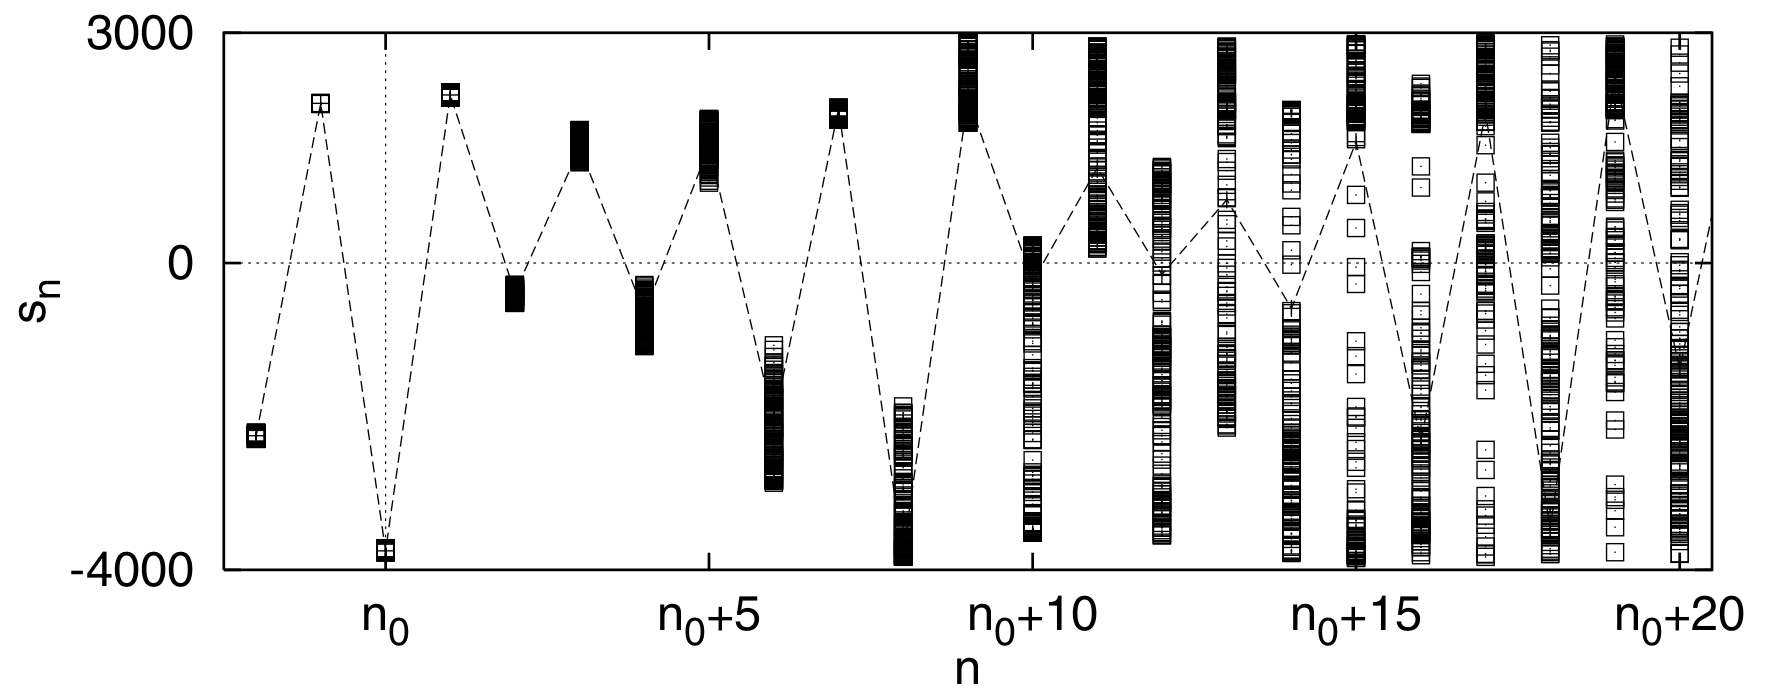
\includegraphics[scale=0.19]{160seg.png} 
	\end{center}
	
\end{frame}

\begin{frame}{Dependencia sensible a las condiciones iniciales.}
	\begin{block}{Observaciones}
		\begin{itemize}
			\item \textit{'causas similares producen efectos similares'} no es válido en sistemas caóticos
			\item No tiene nada que ver con alguna influencia no observada desde fuera del sistema
		\end{itemize}
	\end{block}
	
	\begin{block}{En general}
		Trayectorias cercanas se separan de manera \textit{exponencial} en el tiempo
	\end{block}
\end{frame}

\section{Divergencia exponencial}
\begin{frame} 
\tableofcontents[currentsection] % Solo muestra la sección actual
\end{frame}


\begin{frame}{\textit{Lyapunov}}
	\begin{block}{Aclaración}
		Hablamos de caos únicamente si la separación entre \textit{trayectorias cercanas} ocurre de manera \textbf{\textit{exponencialmente rápida}}
	\end{block}
	
	\begin{block}{Exponente de Lyapunov}
		El exponente promediado adecuadamente de este crecimiento es característico del sistema subyacente a los datos y cuantifica la intensidad del caos. A este se le llama el \textit{\textbf{exponente de Lyapunov}}
	\end{block}
\end{frame}

\begin{frame}{Divergencia de trayectorias del láser NMR}
	\centering
	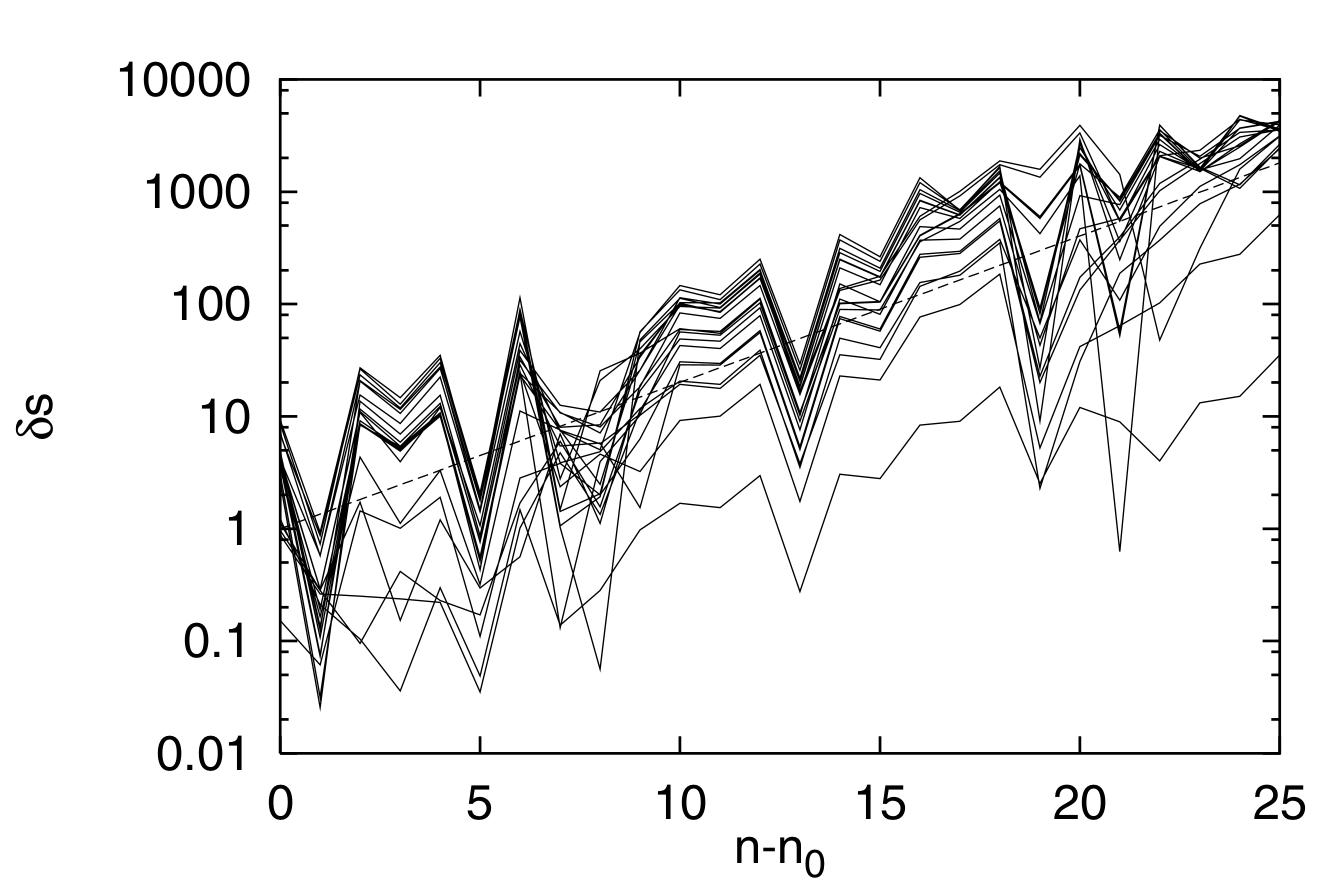
\includegraphics[scale=0.2]{trayectorias.png} 
\end{frame}

\begin{frame}{¿Cómo se determina $\lambda$?}
	\begin{block}{}
		Sean $\mathbf{s}_{n_1}$ y $\mathbf{s}_{n_2}$ dos puntos en el \textit{espacio de fases} cuya distancia $\|\mathbf{s}_{n_1} - \mathbf{s}_{n_2}\| = \delta_0 \ll 1$. Denotemos por $\delta_{\Delta n}$ la distancia, un tiempo $\Delta n$ después, entre las dos trayectorias que emergen de estos puntos: $\delta_{\Delta n} = \|\mathbf{s}_{n_1+\Delta n} - \mathbf{s}_{n_2+\Delta n}\|$. Entonces, $\lambda$ se determina mediante la relación  
		\begin{equation}
			\delta_{\Delta n} \simeq \delta_0 e^{\lambda \Delta n}, \qquad \delta_{\Delta n} \ll 1, \qquad \Delta n \gg 1.
		\end{equation}
	\end{block}
\end{frame}

\begin{frame}{¿Qué indican los valores de $\lambda$?}
	Si asumimos que sólo existe un error aditivo de medición, podemos intentar estimar el \textbf{\textit{exponente de Lyapunov}} de un sistema determinista subyacente asumido
	\begin{block}{Posibles tipos de movimiento y los correspondientes exponentes de Lyapunov.}
		\begin{table}[h!]
		\centering
		\begin{tabular}{ll}
			\hline\hline
			\textbf{Tipo de movimiento} & \textbf{Exponente de Lyapunov máximo} \\
			\hline
			punto fijo estable & $\lambda < 0$ \\
			ciclo límite estable & $\lambda = 0$ \\
			caos & $0 < \lambda < \infty$ \\
			ruido & $\lambda = \infty$ \\
			\hline\hline
		\end{tabular}
		\end{table}
	\end{block}
\end{frame}

\begin{frame}{Motivante para encontrar $\lambda$}
	\begin{block}{Invarianza de $\lambda$}
		Los \textbf{\textit{exponentes de Lyapunov}} son \textit{invariantes} bajo transformaciones suaves de los datos.
	\end{block}
\end{frame}

\section{Medición del exponente máximo a partir de datos}
\begin{frame} 
\tableofcontents[currentsection] % Solo muestra la sección actual
\end{frame}

\begin{frame}{¿Cómo lo medimos?}
	Dado que un exponente de Lyapunov máximo positivo es una fuerte señal de caos, resulta de gran interés determinar su valor para una serie temporal dada
	\begin{block}{Algoritmos con ese propósito}
		\begin{itemize}
			\item \textit{Wolf et al.} (1985)
			\item \textit{Sano \& Sawada} (1985) 
			\item \textit{Eckmann et al.} (1986)
		\end{itemize}		
	\end{block}
	\begin{block}{Algoritmo que vamos a ver}
		Aquí queremos describir un algoritmo introducido por \textit{Rosenstein et al.} (1993) y por \textit{Kantz} (1994) de manera independiente.
	\end{block}

\end{frame}

\begin{frame}{¿Cómo lo medimos?}
	\begin{block}{Algoritmo de \textit{Rosenstein} y \textit{Kantz}}
		Este algoritmo prueba directamente la divergencia exponencial de trayectorias cercanas, y por tanto nos permite decidir si realmente tiene sentido calcular un exponente de Lyapunov para un conjunto de datos dado.
	\end{block}
\end{frame}

\begin{frame}{Algoritmo de \textit{Rosenstein} y \textit{Kantz}}
	\small
	\begin{block}{Paso a paso}
		\begin{enumerate}
			\item Se elige un punto $s_{n_0}$ de la serie temporal en el espacio embebido 
			\item Se seleccionan todos los vecinos con distancia menor que $\epsilon$
			\item Se calcula el promedio sobre las distancias de todos los vecinos al punto de referencia de la trayectoria como función del tiempo relativo $\Delta n$
			\item Repitiendo esto para muchos valores de $n_0$, las fluctuaciones de las tasas de expansión efectivas se promediarán.
		\medskip
				
		Así, se debe calcular:

		\begin{equation}
			(\Delta n) = \frac{1}{N} \sum_{n_0=1}^{N} \ln \left( \frac{1}{|\mathcal{U}_\epsilon(s_{n_0})|} \sum_{s_n \in \mathcal{U}_\epsilon(s_{n_0})} |s_{n_0+\Delta n} - s_{n+\Delta n}| \right)
		\end{equation}
		\end{enumerate}
	\end{block}

\end{frame}

\begin{frame}{Algoritmo de \textit{Rosenstein} y \textit{Kantz}}
	\begin{block}{Observaciones}
		\begin{itemize}
			\item Como no se conocen ni la dimensión mínima de embebido $m$ ni la distancia óptima $\epsilon$, se debe calcular $S(\Delta n)$ para varios valores de ambos parámetros
			\item El tamaño de la vecindad debe ser lo más pequeño posible, pero lo suficientemente grande como para que en promedio cada punto de referencia tenga al menos unos pocos vecinos
			\item Si para cierto rango de $\Delta n$ la función $S(\Delta n)$ muestra un incremento lineal \textit{robusto}, su pendiente es una estimación del exponente de Lyapunov máximo $\lambda$ por paso temporal
		\end{itemize}
	\end{block}

\end{frame}



\end{document}